\chapter{Must Have Concepts}
\label{chapter:must_have_concepts}
During this chapter, the author will discuss topics that help understand the technological developments along this thesis project. The developments will involve both hardware and software components. As such, there are hardware and software concepts that are important to have before discussing the following chapters.

The candidate will develop a \acrshort{soc} in this project. However, he will not create it from scratch. The candidate will use the \textit{IOb-SoC} as a starting point. Consequently, it is important to understand how the \textit{IOb-SoC} works beforehand. It is also important to study the \textit{RISC-V} \acrfull{isa}. Since the hardware developed in this project will be compatible with the \textit{RISC-V} \acrshort{isa}. Furthermore, the software developed will be cross-compiled with the \textit{RISC-V} toolchain. An important part when developing a system is its testing and simulation before implementation. Therefore, the author will review the available methods for simulating the developed components. Lastly, an important concept for this project is the boot flow of an \acrfull{os} on a \textit{RISC-V} platform.

\section{The \textit{IOb-SoC} platform}
\label{section:the_iob_soc_template}
The \textit{IOb-SoC}~\cite{iob_soc_repo} is a System-on-Chip (SoC) template that eases the creation of a new SoC. The \textit{IOb-SoC} provides a base Verilog hardware design equipped with an open-source \textit{RISC-V} processor, an internal SRAM memory subsystem, a UART, and an optional interface to external memory. If the external memory interface is selected, the \textit{IOb-SoC} will include an instruction L1 cache, a data L1 cache and a shared L2 cache. The L2 cache communicates with a third-party memory controller IP (typically a DDR controller) using an AXI4 master bus. Users can add IP cores and software to build their own SoCs quickly. This way, hardware accelerators can be easily created and tested with the developed firmware.

In figure \ref{fig:bd_original} it is represented a sketch of the \acrshort{soc} design. This design is valid at the start of this project. During the hardware developed chapter \ref{chapter:hardware_developed} some alterations were made to the \textit{IOb-SoC} original template.

\begin{figure}[!h]
    \centering
    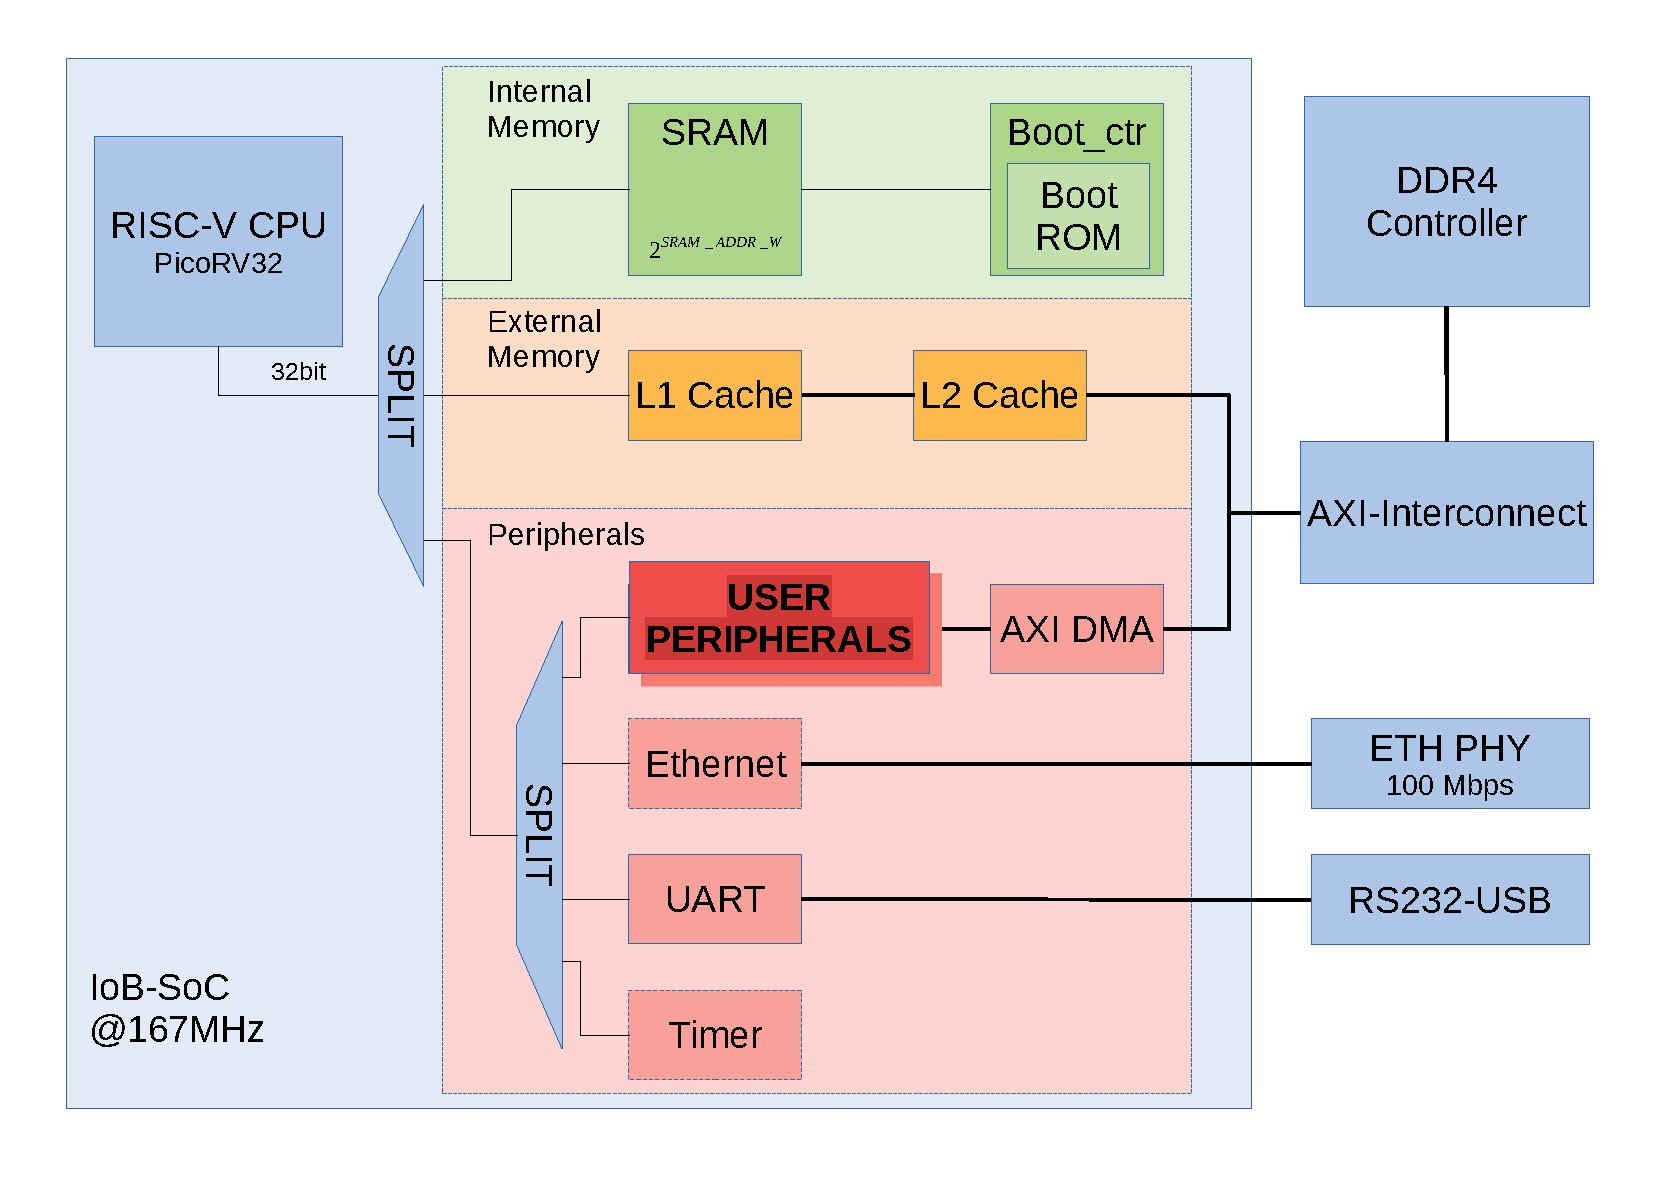
\includegraphics[width=0.7\linewidth]{bd_original.pdf}
    \caption{\textit{IOb-SoC} sketch.}
    \label{fig:bd_original}
\end{figure}

Building a new processor-based system from scratch can be difficult. The \textit{IObundle} developers created the \textit{IOb-SoC} to facilitate this process. This work develops a variant of the existing \textit{IOb-SoC} capable of running a Linux Operating System. \textit{IOb-SoC} currently supports two FPGA board models: the Xilinx Kintex UltraScale KU040 Development Board and the Cyclone V GT FPGA Development Kit.

\subsection{\textit{IOb-SoC} \textit{Makefiles}}
\textit{Makefiles} are essential because they allow automating processes. This way, instead of executing multiple lines to achieve a goal, the user can run a single command. That command will execute a \textit{Makefile} script that runs the multiple processes needed to achieve a specific goal without specifying them. For example, to run a simulation, a developer using this project \acrshort{soc} would only have to write in the terminal the commands in listing~\ref{lst:run_simulation}.

\begin{lstlisting}[language=make, caption={Run a simulation.}, label=lst:run_simulation]
    make sim-clean
    make sim-run
\end{lstlisting}

The first command in listing~\ref{lst:run_simulation} cleans all the files related to a previous simulation execution. Then the second command runs a new simulation. This simulation will use the default configurations in the \enquote{config.mk} file. A \textit{Makefile} target follows each of the \enquote{make} commands. A target is a section of the \textit{Makefile} that may or may not depend on other targets and executes a sequence of commands. In the example~\ref{lst:run_simulation} there are two targets, \enquote{sim-clean} and \enquote{sim-run}.

The main \textit{Makefile} in \textit{IOb-SoC} is located at the \textit{IOb-SoC} root directory. The main \textit{Makefile} contains targets that call other \textit{Makefiles} and sets the values for the default frequency, baud rate, \acrshort{fpga} board used and simulator used. The \textit{Makefiles} the main one can call are at the \textit{IOb-SoC} \acrshort{fpga} boards, simulators, firmware, \enquote{PC} emulation or documentation directory. Each directory in \textit{IOb-SoC} contains a \enquote{*.mk} file which holds \enquote{make} variables and targets that complement the \textit{Makefiles}. The \textit{IOb-SoC} \textit{Makefiles} can include only the \enquote{*.mk} they need.

When executing the command \lstinline[language=bash]{make sim-run} the computer will run the \enquote{run} target of the \textit{Makefile} in the default simulator directory. The simulator \textit{Makefile} will include the \enquote{simulator.mk}, \enquote{hardware.mk} and \enquote{config.mk} files. The \enquote{simulator.mk} file is common to all simulators. Both \acrshort{fpga}s and simulators \textit{Makefiles} include the \enquote{hardware.mk} file. The \enquote{hardware.mk} file includes all the hardware modules that the \acrshort{soc} uses. Lastly, the \enquote{config.mk} is located at the \textit{IOb-SoC} root directory and all \textit{Makefiles} use it. The \enquote{config.mk} defines the \enquote{make} variables that are important for hardware and software, for example which peripherals the \acrshort{soc} contains.

\subsection{\textit{IOb-SoC} peripherals}
Developers add the \textit{IOb-SoC} peripherals under the submodules directory in the \textit{IOb-SoC} folder. Inside the submodules directory there exists a folder for each of the peripherals. Furthermore, the \acrshort{cpu}, the \enquote{iob_cache} module, the \enquote{iob_mem} hardware, the \enquote{iob_axi} interface and the \textit{iob-LIB} repository can also be found in the submodules directory. The \textit{IObundle} engineers developed the \textit{iob-LIB} submodule for it to contain small generic hardware modules and software script used in \textit{IOb-SoC}.

All the submodules may contain hardware and software components. For each hardware peripheral it is recommended to develop a set of bare metal firmware functions that allow to use the peripheral with the \acrshort{soc} without an \acrshort{os}. Since the \textit{IOb-SoC} platform also allows to emulate the developed firmware in the users personal computer, the peripherals should have software function that emulate its firmware drivers.

The peripheral should have the following \enquote{*.mk} files to integrate it into \textit{IOb-SoC}:
\begin{itemize}
    \item the \enquote{PERIPHERAL_REPO/hardware/hardware.mk} so the user can add the peripheral hardware modules to the \acrshort{soc}.
    \item the \enquote{PERIPHERAL_REPO/software/embedded/embedded.mk} allows the user to use the peripheral firmware drivers.
    \item the \enquote{PERIPHERAL_REPO/software/pc-emul/pc-emul.mk} permits to emulate the peripheral behaviour in the users' computer.
\end{itemize}
The developer has to include the \enquote{PERIPHERAL_REPO/hardware/hardware.mk} file in the \textit{IOb-SoC} \enquote{hardware.mk} file. He can include it by adding \lstinline[language=make]{include $(PERIPHERAL_DIR)/hardware/hardware.mk} to the \textit{IOb-SoC} \enquote{hardware.mk}. In the firmware \textit{Makefile} the develops has to include the \enquote{PERIPHERAL_REPO/software/embedded/embedded.mk} file to use the peripheral drivers. Lastly in the \enquote{pc_emul} \textit{Makefile} he has to include the \enquote{PERIPHERAL_REPO/software/pc-emul/pc-emul.mk} file.

In the \enquote{config.mk} file, located in the \textit{IOb-SoC} repository root, the developer needs to add the \enquote{PERIPHERAL_REPO} to the \enquote{PERIPHERALS} \enquote{make} variable and create a variable that indicates the peripheral directory. The user should define the variable that indicates the peripheral directory similarly to: \lstinline[language=make]{PERIPHERAL_REPO_DIR=$(ROOT_DIR)/submodules/PERIPHERAL_REPO}.

The peripheral also needs the following files to be automatically instantiated in the \acrshort{soc} hardware: \enquote{inst_tb.vh}, \enquote{inst.vh} and \enquote{pio.vh}. The \textit{Makefiles} use the \enquote{inst_tb.vh} file to add the needed verilog to the testbench core for the system to simulate. It uses the \enquote{inst.vh} to instantiate the peripheral hardware module in the \textit{IOb-SoC} core. Finally, the \enquote{pio.vh} file contains which input and outputs signals that should be added to the system core hardware. Those files should be in the \enquote{PERIPHERAL_REPO/hardware/include} directory. Listing \ref{lst:inst_file} presents an example of the \enquote{inst.vh} contents.


\begin{lstlisting}[language=Verilog, caption={Example of the \enquote{inst.vh} file.}, label=lst:inst_file]
//
// TIMER
//
iob_timer timer
  (
   .clk      (clk),
   .rst      (reset),

   //cpu interface
   .valid(slaves_req[`valid(`TIMER)]),
   .address(slaves_req[`address(`TIMER,`TIMER_ADDR_W+2)-2]),
   .wdata(slaves_req[`wdata(`TIMER)]),
   .wstrb(slaves_req[`wstrb(`TIMER)]),
   .rdata(slaves_resp[`rdata(`TIMER)]),
   .ready(slaves_resp[`ready(`TIMER)])
   );
\end{lstlisting}

\subsection{Internal Buses}
Review the \enquote{cpu\_i\_resp}, \enquote{cpu\_d\_resp}, \enquote{cpu\_i\_req} and \enquote{cpu\_d\_req} signals.
%define WSTRB_W `WSTRB_W_(DATA_W)
%define WRITE_W `WRITE_W_(DATA_W)
%define READ_W  `READ_W_(DATA_W)
%define WDATA_P `WDATA_P_(DATA_W)
%define ADDR_P  `ADDR_P_(DATA_W)
%define VALID_P `VALID_P_(ADDR_W, DATA_W)
%define REQ_W  `REQ_W_(ADDR_W, DATA_W)
%define RESP_W `RESP_W_(DATA_W)
%define req(I)       `req_(I, ADDR_W, DATA_W)
%define resp(I)      `resp_(I, DATA_W)
%define valid(I)     `valid_(I, ADDR_W, DATA_W)
%define address(I,W) `address_(I, W, ADDR_W, DATA_W)
%define wdata(I)     `wdata_(I, ADDR_W, DATA_W)
%define wstrb(I)     `wstrb_(I, ADDR_W, DATA_W)
%define write(I)     `write_(I, ADDR_W, DATA_W)
%define rdata(I)     `rdata_(I, DATA_W)
%define ready(I)     `ready_(I, DATA_W)

\subsection{\textit{iob-split} and \textit{iob-merge}}
The \textbf{\textit{iob-split}} is simply a configurable \acrfull{demux}. Meaning that when the \textit{iob-split} hardware module is instantiated the developer can configure it. The developer is able to change the size of the \acrlong{demux} and the selection bits, through N\_SLAVES and P\_SLAVES respectively. N\_SLAVES corresponds to the number of slaves, witch can also be seen as the number of the \acrshort{demux} outputs. P\_SLAVES indicates the slave select word \acrfull{msb} position, in other words it is the position of the \acrshort{msb} of the \acrlong{demux} selection bits. The number of the selection bits is given by equation \ref{eq:number_bits}.

\begin{equation}
    \label{eq:number_bits}
    Nb = log_2(N\_SLAVES)+(log_2(N\_SLAVES)==0)
\end{equation}

The \textbf{\textit{iob-merge}} works similar to the \textit{iob-split} but instead of being a \acrshort{demux} it is a configurable \acrfull{mux}. Meaning that instead of having multiple outputs and one input it has multiple inputs and one output. The number of inputs is indicated by N\_SLAVES and the selection bits are chosen by P\_SLAVES.

\subsection{Bootloader and bare-metal firmware}
%\subsection{Old simulation testbench}

\section{\textit{RISC-V}}
\label{section:riscv}
Talk about the 32 registers in the register file

The instruction each ISA extension contains...

\acrfull{csr} needed to run a full feature OS... (core\_id, misa, mcause, ...)

\subsection{CLINT Specification}
The \textit{RISC-V} \textbf{CLINT} is described ...
Platform must support an ACLINT MTIME counter resolution of 100ns or less (corresponding to a clock tick frequency of at least 10 MHz).

\subsection{PLIC Specification}
The \textit{RISC-V} \textbf{PLIC} was first described in the privilege instructions documentation, but since version 1.10 it was moved to its own document.

\subsection{UART/Serial Console}
\label{section:serial_console}
In the \textit{RISC-V} Platform Specification~\cite{riscv_platform_specification} it is defined that every embedded \acrfull{os} is required to have a \acrshort{uart} port implementation that is register-compatible with the industry standard \textit{UART 16550}, which was studied in chapter~\ref{section:uart16550}. The \textit{UART 16550} already exists for a long time, it was released by \textit{National Semiconductor} in 1987, and is present and supported by a large number of software and hardware. The \textit{UART 16550} is often used connected to an RS-232 interface and in this project the development boards used are connected through RS-232 to the computer.

The \textit{UART 16550} registers are...

\section{The Linux Boot Flow on \textit{RISC-V}}
\label{section:linux_boot_flow}
\subsection{Bootloader firmware}
OpenSBI
\subsection{What is a device tree?}

\section{Open Source Verification tools}
\label{section:verification_tools}
Verification tools are ....

https://www.sifive.com/blog/risc-v-qemu-part-1-privileged-isa-hifive1-virtio

\subsection{Hardware logic simulators}
For testing purposes, it is important to have a good hardware simulation environment. For that, we take advantage of already existing and well-developed tools. There exist a number of simulation tools, most of them are proprietary, as for example \textit{xcelium} from \textit{Candence}. Its utilization can increase the cost of a project significantly. In this Thesis we will make an effort of using open-source, free to use, verification tools. In specific, we will take advantage of \textit{Icarus Verilog} and \textit{Verilator}. Although both tools are for verification, they serve different purposes, due to their characteristics.

\begin{itemize}
    \item \textbf{\textit{Icarus Verilog}} is a Logic Simulator that uses verilog or system-verilog testbenchs to test the UUT (Unit Under Test). Unfortunately, its support for system-verilog is limited and some designs might not run in this simulator. \textit{Icarus Verilog} is also known as \textit{IVerilog}.
    
    After compiling the hardware design, \textit{IVerilog} outputs a file which can be run line by line to simulate designed logic.
    
    \item \textbf{\textit{Verilator}} transforms the \textit{Verilog} \acrshort{hdl} designs into a \textit{C++} program that can be executed after being compiled. Using \textit{C++} to create a testbench allows to execute the converted hardware program as a normal program. This way simulating the hardware initially described in \textit{Verilog}. While also allowing to easily make use of system calls. The testbench needed to run with Verilator is similar to the testbench in \textit{Verilog} used with \textit{Icarus}.
\end{itemize}

\textbf{The biggest differences} are: \textit{Verilator} only represents logic signal as 1's or 0's, contrary to \textit{IVerilog} which also represents unknown values as X's; Since \textit{Verilator} ends up being a C++ program it is much faster to run the simulation than with \textit{IVerilog}; On another perspective \textit{Verilator} is slower than \textit{IVerilog} to interpret the hardware logic design.
As such, it is easier to use \textit{IVerilog} to detect errors on the design, but it is better to use \textit{Verilator} for more complexed simulations.

\subsection{Qemu Simulation}
QEMU is an open-source machine emulator and virtualizer, allowing running software and firmware, like operating systems and Linux distributions on many different devices and architecture using a personal computer. It is similar to VMware or VirtualBox. QEMU is a functional emulator; it translates the instructions that were supposed to run on the target architecture to instructions that run on the host CPU. Other types of emulators are Trace-accurate, like Spike, and Cycle-accurate, for example, Verilator. The advantage of using a functional emulator like QEMU is that it is way faster than the other emulation types. A functional emulator runs 100 million to > 1 billion instructions per second, while trace-accurate or cycle-accurate run 10 to 100 thousand instructions per second.

Emulating Linux in \textit{RISC-V} with QEMU is helpful to create and test software for \textit{RISC-V} platforms. QEMU can be used to emulate both 32-bit and 64-bit \textit{RISC-V} CPUs. During this work, an implementation of the Linux kernel will be tested on QEMU running on a \textit{RISC-V} board. The platform that is going to be used is the \textit{virt} board. Virt is a board that does not contain any real hardware but is designed to be used in virtual machines. To define which board the emulation is supposed to run in when calling QEMU, the following argument should be passed: \textit{--machine virt}.
